
% In the plots:
% consistent colours?
% max(m-1) -> m-1

% Check with Matthias:
% * c.f. = compare with (like ie, eg) is that ok to use?
% * periodic behaviour of dtn in LLG case: why does it matter that we are using cartesian coordinates?


% Check with Milan:
% why is TR dt growing slower in stiff example? ringing? citation?


% Fixup ebdf3 code and include in oomph-lib

\chapter{An adaptive implicit midpoint rule scheme}
\chaptermark{Adaptive IMR}
\label{sec:adaptive-imr}


The implicit midpoint rule (IMR) is a well known integration scheme for initial value ordinary differential equations (ODEs) with favourable stability and accuracy properties (see \cref{sec:time-discretisation} or \cite[204]{HairerNorsettWanner}).
It also has beneficial ``geometric integration'' properties when applied to the time integration of the Landau-Lifshitz-Gilbert equation (discussed in
\cref{sec:ensuring-constant-mv,sec:energy-cons}) and energy conservation properties when applied to the semi-discretised Navier-Stokes equations \cite{Sanderse2013}.
However it is a non-trivial task to create an efficient adaptive time step selection algorithm for the IMR using typical approaches.

In \thisref{sec:adaptive-imr} we describe a novel adaptive IMR algorithm based on efficient estimates of the local truncation error by an explicit step.
We then demonstrate the effectiveness of this algorithm on a number of ODE test problems in \cref{sec:aimr-testing} and an ODE form of the LLG in \cref{sec:imr-ode-llg-numer-exper}.
Experiments on a full PDE LLG problem are performed in \cref{cha:numer-experiments}.


\section{Fixed step size implicit midpoint rule}
\label{sec:fixed-step-implicit}

Let $\yv(t)$ be a vector function and denote an approximation to $\yv(t)$ at $t = t_n$ by $\yv_n$.
Let $\dtn = t_{n+1} - t_n$ be the $n$th time step (or just ``step'').
Then, given a system of ordinary differential equations (ODEs) of the form
\begin{equation}
  \yv'(t) = \ffv{t, \yv(t)},
  \label{eq:43}
\end{equation}
the implicit midpoint rule (IMR) is
\begin{equation}
    \yv_{n+1} = \yv_n + \dtn \ffv{\frac{t_{n+1} + t_n}{2}, \frac{\yv_n + \yv_{n+1}}{2}}.
    \label{eq:67}
\end{equation}

We introduce shorthand notation for the midpoint values of $t$ and $\yv$:
\begin{equation}
  \begin{aligned}
    \thf & = \frac{t_{n+1} + t_n}{2} \quad \bigb{= t_n + \frac{\dtn}{2}}, \\
    \yvm &= \frac{\yv_{n+1} + \yv_n}{2}.
  \end{aligned}
\end{equation}
In this notation the IMR is
\begin{equation}
  \yv_{n+1} = \yv_n + \dtn \ffv{\thf, \yvm}.
  \label{eq:basic-midpoint}
\end{equation}

The IMR can also be written in the standard form for implicit Runge-Kutta methods as
\begin{equation}
  \begin{aligned}
    k_1 &= \ffv{t_n + \frac{1}{2} \dtn, \yv_n + \frac{1}{2} k_1}, \\
    \yv_{n+1} &= \yv_n + 1 \cdot \dtn k_1,
  \end{aligned}
\end{equation}
which is equivalent to the Butcher tableau \cite[135]{HairerNorsettWanner} shown in \cref{tab:butcher-imr}.

\begin{table}
  \begin{equation*}
    \begin{array}{c|c}
      \frac{1}{2}  &     \frac{1}{2}  \\
      \hline
                   & 1 \\
    \end{array}
  \end{equation*}
  \caption{The Butcher tableau for the implicit midpoint rule.}
  \label{tab:butcher-imr}
\end{table}

Note that, unlike for multistep methods, \cref{eq:basic-midpoint} is valid for both constant and variable step sizes, because there is no dependence on previous steps.


\section{Adaptive implicit midpoint rule}
\label{sec:adapt-impl-midp}

Adaptive time step selection algorithms are typically based on approximating the local truncation error (LTE), the error due to a single step of the integration scheme (see \cref{sec:deriv-local-trunc}).
These estimates can be used to select appropriate time steps such that the LTE remains close to a specified value.
In \thisref{sec:adapt-impl-midp} we first discuss why the standard approaches used to estimate the LTE fail for the IMR, and the approach that we will use.
We next derive the formulae required and discuss how a complete adaptive time step selection algorithm can be implemented using the LTE estimates.
Finally we mention a limitation of the scheme when applied to certain problems.

\subsection{Construction of an LTE estimate}

Due to the complexity of the LTE of the implicit midpoint rule there are difficulties with the Milne-device approach described in \cref{sec:adaptivity}.
In particular, the LTE of IMR has a term involving the error due to the approximation $\yv(\thf) \sim \yvm$ (term II of \cref{eq:trunc-mid}).
In order to perform the algebraic rearrangements to obtain the LTE using a Milne-device-like approach we would need this term to appear in the LTE of the predictor.
However it can only appear in the LTE expression for a time integrator which uses the midpoint approximation for $\yv$.
It turns out that the only such second order time integrator is IMR itself.\footnote{To see why this is the case }
So this term of the error is difficult to approximate using a Milne-device-like method.

An alternative approach, commonly used in Runge-Kutta time integrators, is to repeat the calculation using a higher order method and compare the two answers to directly obtain an LTE estimate \cite[165]{HairerWanner}.
However evaluations of the derivative function ($\fv$ in \cref{eq:43}) are expensive, and the calculation of a single step of a high order Runge-Kutta method requires a number of such evaluations.
Hence such approaches usually rely on pairs of Runge-Kutta methods which share most of their derivative evaluation points but have different orders of accuracy.
These are known as embedded Runge-Kutta methods, a widely used example is the Dormand–Prince pair (order 4/5) used in MATLAB's \texttt{ode45} function \cite{matlab-ode45}.

Unfortunately there is no third order method which requires only $\ffv{\thf, \yvm}$ and a single other function evaluation.\footnote{IMR's single function evaluation is positioned such that the second order error terms cancel. Adding one additional evaluation cannot retain the symmetry causing this cancellation and so does not increase the order, at least two additional evaluations are needed.}
To get around this problem we instead use a little known explicit version of the third order backwards difference method (eBDF3).
This method only requires three history values and a single explicit function evaluation in order to compute a 3rd-order accurate approximation to $\yv(t_{n+1})$.
Since only one function evaluation is required the computational cost is equivalent to an embedded Runge-Kutta method.
With this approach our estimate for the local truncation error is simply
\begin{equation}
  \label{eq:aimr-lte-est}
  \lte = \yv_{n+1}^{\ebdf} - \yv_{n+1}^\imr + \order{\dtn^4}.
\end{equation}
The eBDF3 method is not widely used because it does not have the basic property essential for time integration \cite[365]{HairerNorsettWanner}:
\begin{equation}
  \lim_{\dtn \rightarrow 0} \bigb{ \max_n \norm{\yv_{n} - \yv(t_n)}} = 0
\end{equation}
which is known variously as ``stability'' \cite[378]{HairerNorsettWanner} or ``convergence'' \cite[6]{Iserles2009}.
However, for our usage the IMR history values are used as input for a \emph{single} step of eBDF3, hence the stability is irrelevant.\footnote{This could also be thought of as an extrapolation to the value of $\yv$ at $t_{n+1}$ using the previous IMR-generated values and a derivative.}
The variable time step version of eBDF3 does not appear in the literature, so we derive the method below in \cref{sec:variable-step-ebdf3} .

Alternatively a 3rd order Adams-Bashforth scheme (AB3) could be used as a predictor, but this would require three previous derivative values instead of $y$ values making the initialisation of the scheme a little more complex and expensive.
Additionally, the calculation of coefficients for the variable step Adams-Bashforth schemes is more complex \cite[400]{HairerNorsettWanner}.
However, in contrast to eBDF3, AB3 is stable which could simplify the process of testing an implementation.


\subsection{The variable step eBDF3 method}
\label{sec:variable-step-ebdf3}

The explicit BDF methods are explicit time integration methods derived using the same techniques as the usual implicit BDF methods.
The idea is to write down a divided difference representation of an interpolating polynomial, $\pv(t)$, through $\yv_i$, $i=n-k+1, \ldots, n+1$ at the appropriate times (simple backward differences can be used for constant time steps, hence the name).
The derivative of the polynomial is then set equal to the derivative function $\ffv{t, \yv}$ at one of the discrete time steps \cite[400]{HairerNorsettWanner}.
Setting $\pv'(t_{n+1}) = \ffv{t_{n+1}, \yv_{n+1}}$ gives the familiar implicit BDF methods.
If we instead set $\pv'(t_{n}) = \ffv{t_{n}, \yv_{n}}$ we obtain the explicit BDF methods (eBDF) \cite[364]{HairerNorsettWanner}.
We now derive the first three eBDF methods.
% The derivation of the implicit BDF methods is shown in \cref{cha:deriv-impl-backw} and may be useful for comparison.

For this purpose we define the Newton divided differences recursively by
\begin{equation}
  \label{eqn:divided-diff}
  \begin{aligned}
    \yv[t_{n+1}] &= \yv_{n+1}, \\
    \yv[t_{n+1}, t_n] &= \frac{\yv[t_{n+1}] - \yv[t_n]}{t_{n+1} - t_n}, \\
    \yv[t_{n+1}, t_n, t_{n-1}] &= \frac{\yv[t_{n+1}, t_n] - \yv[t_n, t_{n-1}]}{t_{n+1} - t_{n-1}}, \\
    \vdots
  \end{aligned}
\end{equation}
The $k$-th Lagrange interpolation polynomial \cite[124]{BurdenFaires}, \cite[400]{HairerNorsettWanner} can be expressed using these as
\begin{equation}
  \label{eqn:divided-diff-intp}
  \begin{aligned}
    \pv_k(t) &= \yv_{n+1} + \sum_{j=1}^k \yv[t_{n+1}, \ldots, t_{n+1-j}] \prod_{i=0}^{j-1} (t - t_{n+1-i}), \\
    &= \yv_{n+1} + \yv[t_{n+1}, t_n](t - t_{n+1}) + \yv[t_{n+1}, t_n, t_{n-1}](t - t_{n+1})(t - t_n) \\
    &\quad + \yv[t_{n+1}, t_n, t_{n-1}, t_{n-2}](t - t_{n+1})(t - t_n)(t - t_{n-1}) + \ldots \\
    &\quad + \yv[t_{n+1}, \ldots, t_{n+1-k}](t-t_{n+1})\cdots(t-t_{n-k}).
  \end{aligned}
\end{equation}
Differentiating \cref{eqn:divided-diff-intp} with respect to $t$, recalling that divided differences are constants and applying the chain rule to the derivative of the product term we obtain
\begin{equation}
  \begin{aligned}
    \pv_k'(t) &= \yv[t_{n+1}, t_n] + \yv[t_{n+1}, t_n, t_{n-1}]\bigb{(t - t_n) + (t - t_{n+1})} \\
    &\quad + \yv[t_{n+1}, t_n, t_{n-1}, t_{n-2}]\bigb{(t - t_n)(t - t_{n-1}) + (t - t_{n+1})(t - t_{n-1}) + (t - t_{n+1})(t - t_n)} \\
    &\quad + \ldots \\
    &\quad + \yv[t_{n+1}, \ldots, t_{n+1-k}]\bigb{(t-t_{n})\cdots(t-t_{n-k}) + \ldots + (t-t_{n+1})\cdots(t-t_{n-k+1})}, \\
    &= \sum_{j=1}^k \yv[t_{n+1}, \ldots, t_{n+1-j}] \sum_{l=0}^{j-1} \prod_{i=0, i \neq l}^{j-1} (t - t_{n+1-i}).
    \label{eq:59}
  \end{aligned}
\end{equation}
Setting $\ffv{t_n, \yv_n} = \pv_k'(t_n)$ results in
\begin{equation}
  \begin{aligned}
    \ffv{t_n, \yv_n} &= \sum_{j=1}^k \yv[t_{n+1}, \ldots, t_{n+1-j}] \sum_{l=0}^{j-1} \prod_{i=0, i \neq l}^{j-1} (t_n - t_{n+1-i}).
  \end{aligned}
\end{equation}
This can be greatly simplified by noticing that the product $ \prod_{i=0, i \neq l}^{j-1} (t_n - t_{n+1-i})$ is zero whenever it contains $i=1$, \ie whenever $j \geq 2$ and $l \neq 1$.
When $j=1$ the only non-zero terms in the sum of products are for $l=0$ and $i=0$, so we only need to consider the case of $l=1$.
This gives
\begin{equation}
  \begin{aligned}
    \ffv{t_n, \yv_n} &= \sum_{j=1}^k \yv[t_{n+1}, \ldots, t_{n+1-j}] \prod_{i=0, i \neq 1}^{j-1} (t_n - t_{n+1-i}), \\
    &= \yv[t_{n+1}, t_n] + \sum_{j=2}^k \yv[t_{n+1}, \ldots, t_{n+1-j}] \prod_{i=0, i \neq 1}^{j-1} (t_n - t_{n+1-i}), \\
    &= \yv[t_{n+1}, t_n] -\dtn \sum_{j=2}^k \yv[t_{n+1}, \ldots, t_{n+1-j}] \prod_{i=2}^{j-1} (t_n - t_{n+1-i}). \\
  \end{aligned}
  \label{eq:ebdf-general}
\end{equation}

For $k=1$ equation \cref{eq:ebdf-general} reduces to
\begin{equation}
  \begin{aligned}
    \fv(t_n, \yv_n) &= \yv[t_{n+1}, t_n] = \frac{\yv_{n+1} - \yv_n}{\dtn}, \\
    \yv_{n+1} &= \yv_n + \dtn f(t_n, \yv_n), \\
  \end{aligned}
\end{equation}
which is the forward Euler method.

For $k=2$ we have
\begin{equation}
  \begin{aligned}
    \fv(t_n, \yv_n) &= \yv[t_{n+1}, t_n] - \dtn \yv[t_{n+1}, t_n, t_{n-1}] , \\
    &=  \frac{\yv_{n+1} - \yv_n}{\dtn}
    - \frac{\dtn}{\dtn + \dtx{n-1}} \bigb{ \frac{\yv_{n+1} - \yv_n}{\dtn} - \frac{\yv_n - \yv_{n-1}}{\dtx{n-1}}}.
  \end{aligned}
\end{equation}
After some algebra this gives
\begin{equation}
  \label{eq:emr-derivation-rearranged}
  \yv_{n+1} = \yv_n + \bigb{1 + \frac{\dtn}{\dtx{n-1}}}\dtn \ffv{t_n, \yv_n}
    - \frac{\dtn^2}{\dtx{n-1}^2}(\yv_n - \yv_{n-1}),
\end{equation}
which is the variable step equivalent of the leapfrog method (explicit midpoint rule) \cite[715]{GreshoSani}.

For larger values of $k$ the complexity of the algebra grows enormously.
Unfortunately we are interested in the case $k=3$ which is:
\begin{equation}
  \begin{aligned}
    \fv(t_n, \yv_n) &= \yv[t_{n+1}, t_n] - \dtn \yv[t_{n+1}, t_n, t_{n-1}] -\dtn \yv[t_{n+1}, t_n, t_{n-1}, t_{n-2}], \\
    &=  \frac{\yv_{n+1} - \yv_n}{\dtn}
    - \frac{\dtn}{\dtn + \dtx{n-1}} \bigb{ \frac{\yv_{n+1} - \yv_n}{\dtn} - \frac{\yv_n - \yv_{n-1}}{\dtx{n-1}}} \\
    &\quad - \frac{\dtn}{\dtn + \dtx{n-1} + \dtx{n-2}}
         \bigs{
           \frac{\frac{\yv_{n+1} - \yv_n}{\dtn} - \frac{\yv_n - \yv_{n-1}}{\dtx{n-1}}}
                {\dtn +\dtx{n-1}}
           -
           \frac{\frac{\yv_{n} - \yv_{n-1}}{\dtx{n-1}} - \frac{\yv_{n-1} - \yv_{n-2}}{\dtx{n-2}}}
                {\dtx{n-1} +\dtx{n-2}}
         }.
  \end{aligned}
  \label{eq:ebdf-3-initial}
\end{equation}
Solving \cref{eq:ebdf-3-initial} for $\yv_{n+1}$ by hand would be complex and extremely error prone.
Instead \cref{eq:ebdf-3-initial} was solved using the \texttt{SymPy} symbolic manipulation library \cite{sympy} (script available online \cite{ebdf3-sympy-script}).
The resulting time integration scheme is:
\begin{equation}
  \label{eqn:ebdf-coeffs}
  \begin{aligned}
    \yv_{n+1} &= b \fv(t_n, \yv_n) + c_n \yv_n + c_{n-1} \yv_{n-1} + c_{n-2} \yv_{n-2}, \\
    b &= \frac{\dtx{n+1}}{\dtn (\dtn + \dtx{n-1})} (\dtx{n+1} + \dtn) (\dtx{n+1} + \dtn + \dtx{n-1}) ,\\
    c_n &= - \frac{ (2 \dtx{n+1} \dtn + \dtx{n+1} \dtx{n-1} - \dtn^{2} - \dtn \dtx{n-1}) }{\dtn^{2} (\dtn + \dtx{n-1})^{2}} (\dtx{n+1} + \dtn) (\dtx{n+1} + \dtn + \dtx{n-1}),\\
    c_{n-1} &= \frac{\dtx{n+1}^{2}}{\dtn^{2} \dtx{n-1}} (\dtx{n+1} + \dtn + \dtx{n-1}) ,\\
    c_{n-2} &= - \frac{\dtx{n+1}^{2} (\dtx{n+1} + \dtn)}{\dtx{n-1} (\dtn + \dtx{n-1})^{2}}.
  \end{aligned}
\end{equation}
For constant time steps the result reduces to: $ b = 3\dtn$, $c_n = -3/2$, $c_{n-1} = 3$ and  $c_{n-2} = -1/2$ which matches the scheme given in \cite[364]{HairerNorsettWanner}.

It should be noted that the calculation of the coefficients in \cref{eqn:ebdf-coeffs} could be disproportionately expensive if the number of $y$-values is small ($\sim 100$ operations assuming no compiler optimisation of the multiplications).
However when used in finite-element or finite-difference calculations the number of $y$-values is at least tens of thousands, so the cost of \cref{eqn:ebdf-coeffs} is trivial by comparison with, for example, the calculation of $\ffv{t_n, \yv_n}$.


\subsection{Computing the next step size}

We use a standard method \cite[268]{GreshoSani} for computing the next step size from the ratio of the LTE estimate and a target local truncation error $\toltt$
\begin{equation}
  \dtx{n+1} = \bigb{ \frac{\toltt}{\lte} }^{\frac{1}{\texttt{order}+1}} \dtn .
\end{equation}
For the implicit midpoint rule this is
\begin{equation}
  \dtx{n+1} = \bigb{ \frac{\toltt}{\abs{\yv_{n+1}^{eBDF3} - \yv_{n+1}^\imr}} }^{\frac{1}{3}}  \dtn.
  \label{eq:next-step-dt}
\end{equation}

We also impose some additional constraints to handle extreme cases.
If the ratio $\frac{\dtx{n+1}}{\dtn}$ is too small, \ie if the step just taken was much too large to attain the desired accuracy, then we reduce the step size by a factor of 2 and repeat the $n$-th step.
We limit $\frac{\dtx{n+1}}{\dtn}$ to 4 to help improve stability.

Note that some alternative strategies try to minimise the number of modifications to the time step size \cite[Chap. 6]{Iserles2009} \cite[Sec. 2.1]{cvode-manual}.
The motivation for this is the use of a modified Newton-Raphson method where the Jacobian is not recalculated at each Newton step.
In the case of ODE solvers this is extremely beneficial, because the Jacobian is usually dense and direct solvers are used to solve it--by keeping the Jacobian constant the number of solves and Jacobian assemblies are greatly reduced.
The downside is a reduction in the convergence speed of the Newton method.
Keeping the step size constant for as long as possible is required here because modifications to the time step cause modifications to the Jacobian.
However for PDE solvers, and in particular for PDE solvers using iterative methods to solve the linear systems there is little-to-no benefit in using this technique: the reduction in convergence speed is more detrimental than the gain of not assembling and solving the additional sparse linear systems \cite[128]{Iserles2009}.


\subsection{The complete algorithm}

Assuming that we have values for $\yv_n$, $\yv_{n-1}$, $\yv_{n-2}$ (these can be obtained \eg by doing a few steps of fixed step IMR) then an outline of the final adaptive IMR algorithm is as follows:
\begin{enumerate}
\item Calculate $\yv_{n+1}^\ebdf$ from $\yv_n$, $\yv_{n-1}$, $\yv_{n-2}$ using eBDF3, \cref{eqn:ebdf-coeffs}.
\item Calculate $\yv_{n+1}$ from $\yv_n$ using IMR, \cref{eq:67} (along with some linear/non-linear solver as appropriate).
\item Calculate $\dtx{n+1}$ from $\yv_{n+1}^\ebdf$, $\yv_{n+1}$ and $\dtn$ using
  \cref{eq:next-step-dt}.
\item If $t > t_{\text{max}}$ then stop, otherwise set $n := n+1$ and go to step 1.
\end{enumerate}

Steps 1 and 2 are interchangeable, but in some cases the value $\yv_{n+1}^\ebdf$ may be useful as an initial guess for the calculation of $\yv_{n+1}$.


\subsection{Application to Implicit ODEs}
\label{sec:extens-impl-odes}

We sometimes wish to solve an ODE where $\yv'(t)$ is only given implicitly as
\begin{equation}
  \ffv{t, \yv(t), \yv'(t)} = 0,
\end{equation}
for example in the Gilbert form of the Landau-Lifshitz-Gilbert equation.\footnote{This use of ``implicit'' is unrelated to the notion of implicitness in the time integration scheme.}

However the eBDF3 predictor used in the adaptive scheme requires a derivative evaluation, which for derivatives which can \emph{only} be defined implicitly requires a non-linear solve.
This is expensive, so for such cases the adaptive method described here is not efficient.
Note that the LLG can be defined explicitly as well as implicitly, so this limitation does not apply to micromagnetics problems (we can simply use the Landau-Lifshitz form for the required derivative evaluation).


\section{Numerical experiments with simple ODEs}
\label{sec:aimr-testing}


% Regenerate data by running (in control_scripts folder):
% ./parameter-sweep.py -p aimr_odes_order_reduction -p aimr_odes --clean
%  Generate and update plots with commands in the plots dir

In \thisref{sec:aimr-testing} we show the results of some initial testing of the proposed adaptive IMR algorithm for some simple ODE examples.
These experiments will allow us to check that the adaptive algorithm selects sensible time steps and that the errors are commensurate with similar schemes.
Numerical experiments with the LLG equation are detailed in \cref{sec:imr-ode-llg-numer-exper}.


\subsection{Implementation details}
\label{sec:aimr-implementation}

We compare the adaptive IMR developed above with two commonly used adaptive implicit time integrators:
\begin{itemize}
\item The adaptive trapezoid rule with an error estimate constructed using Milne's device with the second order Adams-Bashforth method (AB2) \cite[707]{GreshoSani}.
\item Adaptive BDF2, with the error estimate constructed using Milne's device with the variable step leapfrog method (\ie explicit BDF2) \cite[715]{GreshoSani}.
\end{itemize}

All three methods are implemented within the \oomph framework.
To increase relevance to the general non-linear PDE case (\ie the LLG equation) we use exactly the same methods for the solution of the ODEs as used for semi-discretised PDEs.
So we use the Newton-Raphson method with the Jacobian inverted by a linear solver.
One effect of this is that the baseline numerical error as seen by the ODE solver is the tolerance of the Newton-Raphson method rather than the machine accuracy.

Unless otherwise specified all examples in \thisref{sec:aimr-testing} use an absolute Newton tolerance of $\ntol = 10^{-8}$, an initial time step of $\dtx{0} = 10^{-5}$, and an adaptive integrator tolerance of $\toltt = 10^{-4}$.
Any initial conditions required are calculated from the exact solutions.


\subsection{Polynomial example}
\label{sec:imr-polynomial-example}

The first example is an ODE
\begin{equation}
  \begin{aligned}
    f(t,y) &= 2t, \\
    y(0) &= 0.5,
  \end{aligned}
\end{equation}
with the exact solution
\begin{equation}
  y(t) = t^2 + 0.5.
\end{equation}
This problem should be integrated exactly by all of the methods since $\lte \propto y'''(t) \equiv 0$.
The adaptivity algorithm should detect this and increase the time step at the maximum allowed rate.

The results of this experiment are shown in Figure~\ref{fig:imr-poly2-example}.
As expected, all three methods keep the error extremely small (at a level commensurate with the Newton tolerance, $\ntol$) even for extremely large time steps.
The step size increases rapidly for all methods, as expected.
The computed solution does not look much like a polynomial because the distance between output points is so large (due to large time steps).

\begin{figure}
  \centering
  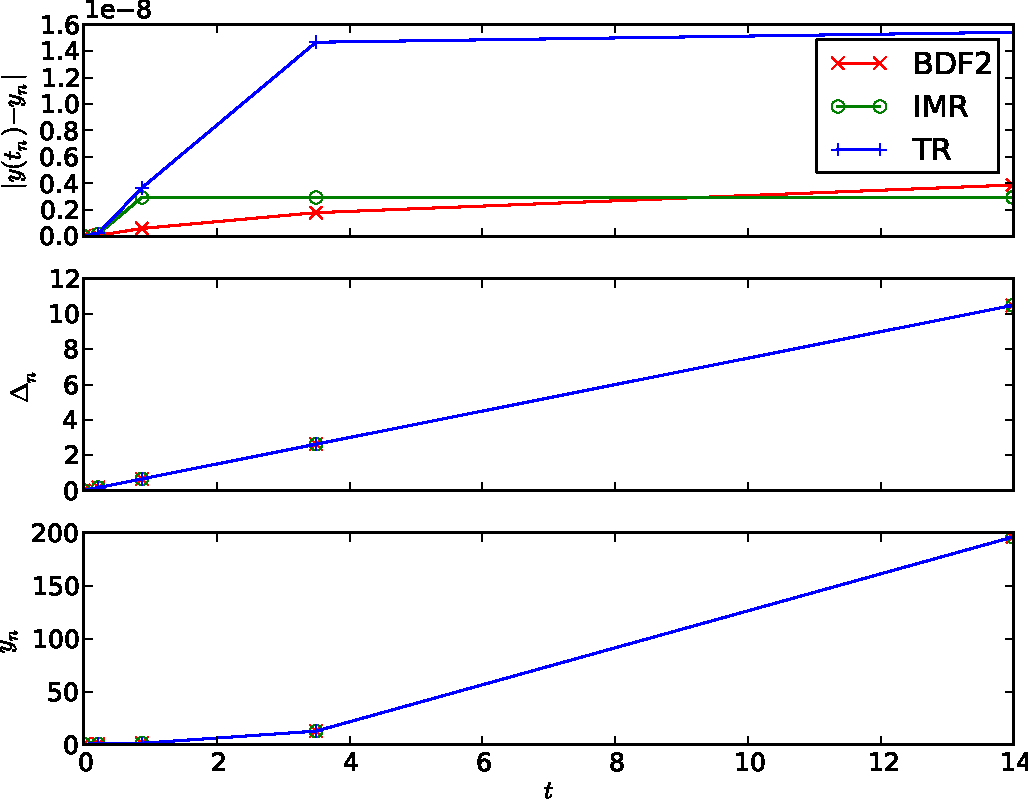
\includegraphics[width=1\textwidth]{plots/aimr_odes_traces/poly2-errornormsvs-dtsvs-tracevaluesvstimes}
  \caption{Absolute error, time step size and computed solutions for the example ODE with exact solution $y(t) = t^2 + 0.5$.}
  \label{fig:imr-poly2-example}
\end{figure}


\subsection{Damped oscillatory example}
\label{sec:oscill-damp-example}

The next test features a damped oscillatory solution, the ODE is
\begin{equation}
  \label{eqn:imr-test-osc-damp}
  \begin{aligned}
    f(t,y) &= - \beta e^{-\beta t} \sin(\omega t) + \omega e^{-\beta t} \cos(\omega t), \\
    y(0) &= 0.
  \end{aligned}
\end{equation}
with the solution
\begin{equation}
  y(t) = e^{-\beta t} \sin(\omega t).
\end{equation}
The adaptive algorithm should produce time steps that oscillate in time with the truncation error, while at the same time gradually increase as the term $e^{-\beta t}$ goes to zero.

\begin{figure}
  \centering 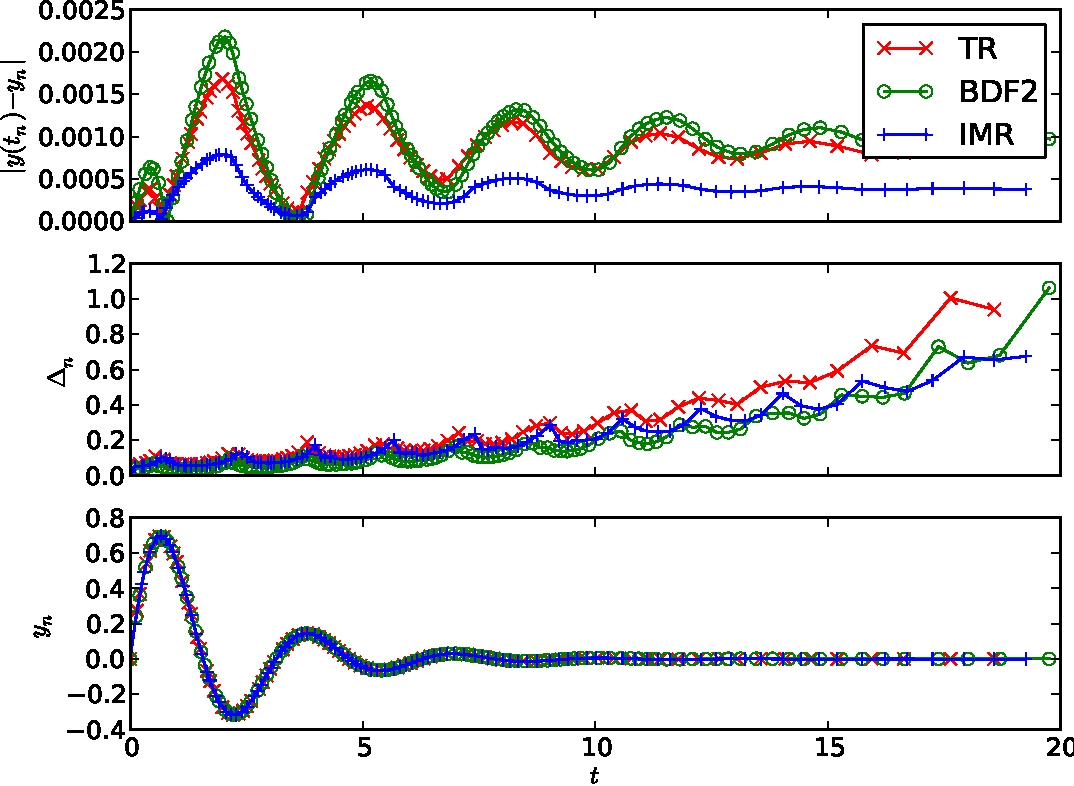
\includegraphics[width=1\textwidth]{plots/aimr_odes_traces/damped_oscillation-errornormsvs-dtsvs-tracevaluesvstimes}
  \caption{Absolute error, time step size and computed solutions for the oscillatory, damped example ODE with exact solution $y(t) = e^{-0.5t} \sin(2\pi t)$.}
  \label{fig:imr-osc-example}
\end{figure}

The ODE was solved with parameters $\omega = 2 \pi$ and $\beta = 0.5$, the results are shown in \cref{fig:imr-osc-example}.
All three methods have similar errors and time step sizes.
The IMR method chooses slightly smaller steps than TR (which explains the slightly lower error magnitudes).
BDF2 has the worst errors as expected because the coefficient of the main LTE term is the largest (see \cref{sec:deriv-local-trunc}).

Note that the plot shows the global error, whereas local truncation error estimates are used for step size selection calculations.
Hence the fact that the global error increases above the tolerance, $\toltt$, is not surprising.

Interestingly, there is a slight lag on the time step response of the IMR method as time steps become larger.
This could be due to the fact that IMR uses data from three previous steps in its LTE estimate, whereas the others only use two previous steps.

In \cref{fig:imr-osc-example-scatter} we show plots of the decrease in global error norm as the tolerance is decreased.
The consistent decrease in the error norms indicates that the all of the adaptive methods are able to control the error in the expected manner.

\begin{figure}
  \centering 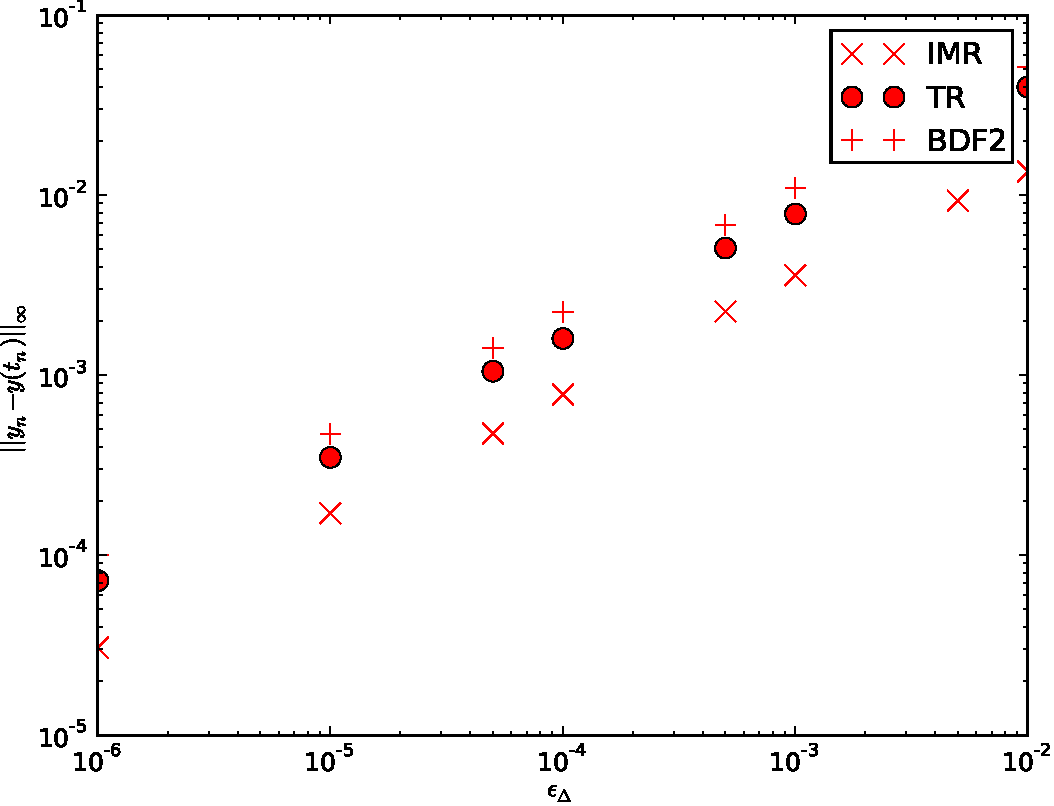
\includegraphics[width=0.8\textwidth]{plots/aimr_odes/damped_oscillation-maxoferrornormsvs-tol}
  \caption{Behaviour of the global error norm with varying tolerance for the oscillatory, damped example ODE with exact solution $y(t) = e^{-\beta t} \sin(\omega t)$.}
  \label{fig:imr-osc-example-scatter}
\end{figure}

\subsection{A stiff problem}
\label{sec:imr-stiff-example}

We consider the stiff example ODE used in the definition of A-stability:
\begin{equation}
  \label{eqn:imr-test-stiff}
  \begin{aligned}
    f(t, \yv) &= -\lambda \yv, \\
    \yv(0) &= 1,
  \end{aligned}
\end{equation}
with the exact solution
\begin{equation}
  \label{eqn:imr-test-stiff-exact}
  \yv(t) = e^{-\lambda t}.
\end{equation}
This example will test that the single step of the eBDF method provides reliable LTE estimates even in cases of extreme stiffness.
The time steps should start small but rapidly increase as the exponential decays to zero.

The results of the applying the three methods to problem~\cref{eqn:imr-test-stiff} with $\lambda = 100$ (fairly stiff) and $\yv_0 = 1$ are shown in \cref{fig:imr-stiff-example}.
The behaviour of the IMR and BDF2 time integrators is essentially the same, indicating that our adaptivity algorithm is effective for stiff problems.
The time steps selected by the TR algorithm do not grow as fast as those selected for the other schemes at large $t$, ??ds this is probably due to the ``ringing'' phenomenon \cite{??ds}.

\begin{figure}
  \centering
  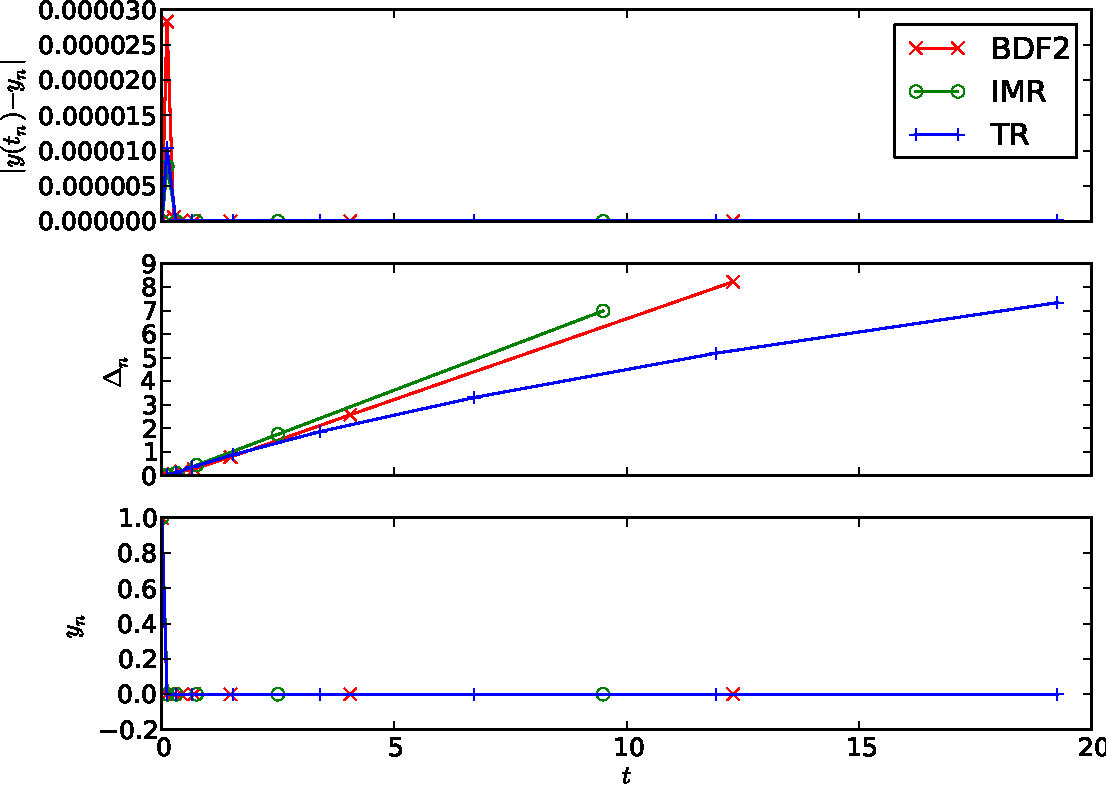
\includegraphics[width=1\textwidth]{plots/aimr_odes_traces/simple_stiff-errornormsvs-dtsvs-tracevaluesvstimes}
  \caption{Absolute error, step size and computed solutions for the stiff example ODE.}
  \label{fig:imr-stiff-example}
\end{figure}


\subsection{Order reduction example}
\label{sec:order-reduct-example}

\begin{figure}
  \centering  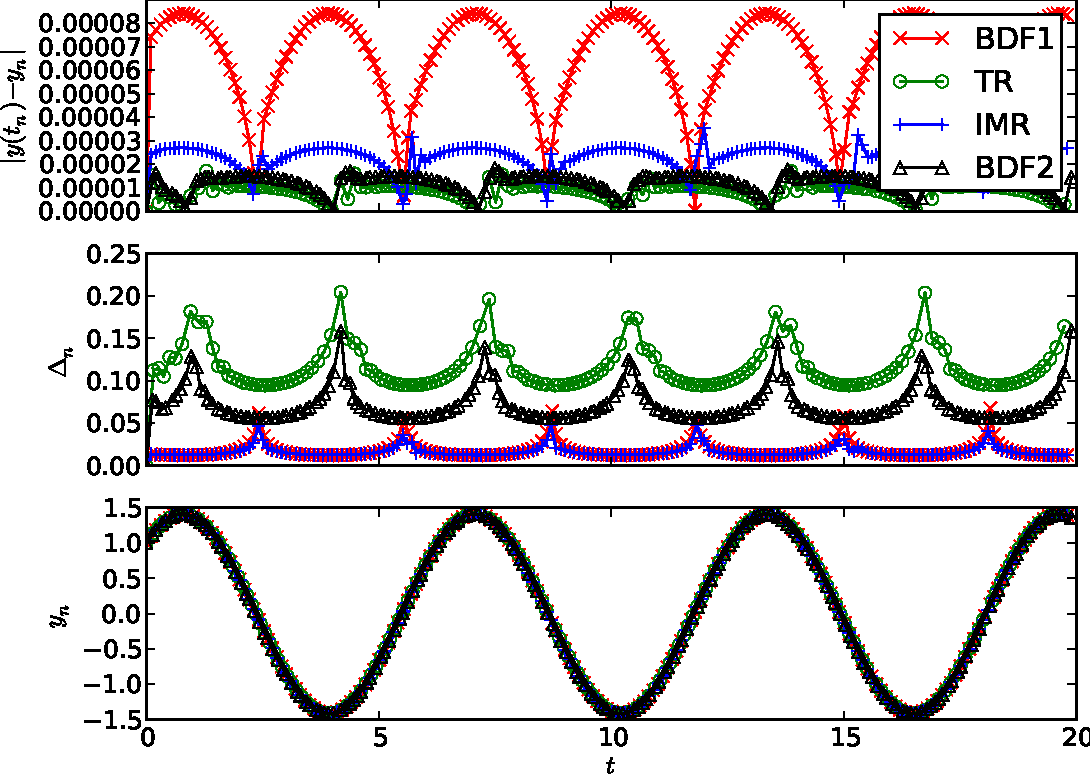
\includegraphics[width=0.8\textwidth]{plots/aimr_odes_traces/strong_order_reduction-errornormsvs-dtsvs-tracevaluesvstimes}
  \caption{Absolute error, step size and computed solutions for the stiff order reduction example ODE given in \cref{eqn:imr-test-order-reduction}.}
  \label{fig:imr-order-reduction-example}
\end{figure}

\begin{figure}
  \centering  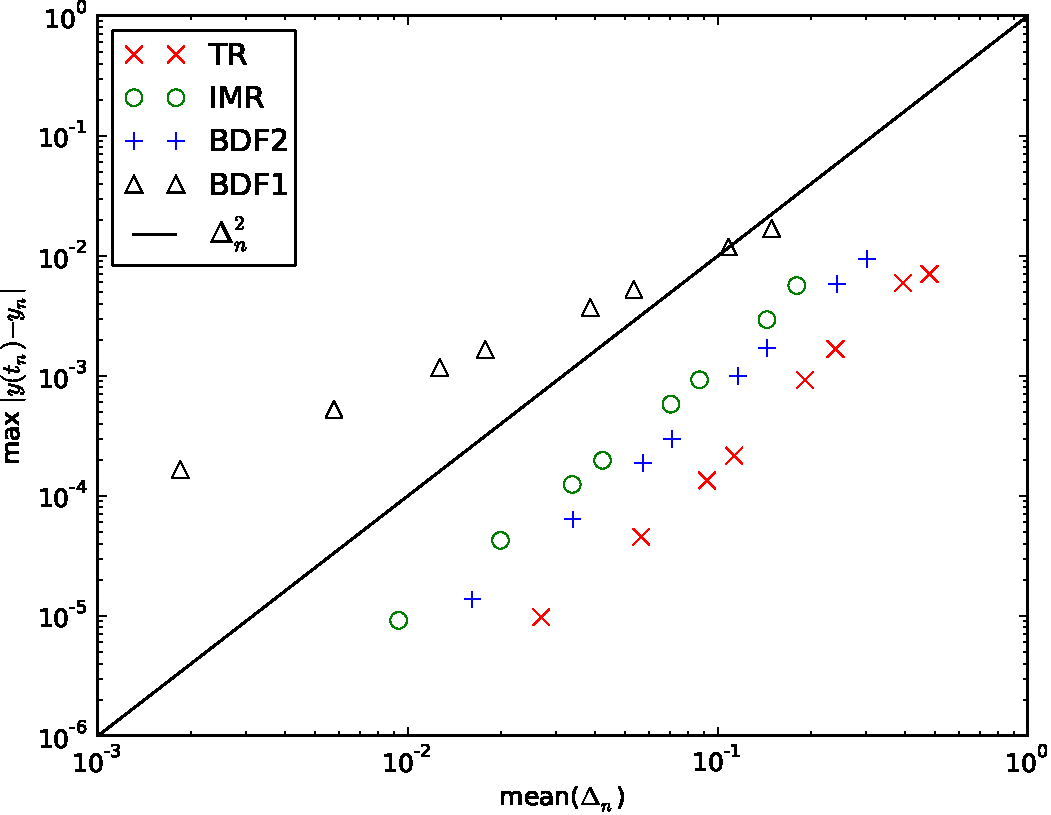
\includegraphics[width=1\textwidth]{plots/aimr_odes/order_reduction-maxoferrornormsvsmeanofdts.pdf}
  \caption{Behaviour of the global error norm with varying tolerance vs mean step size for the order reduction example.}
  \label{fig:imr-order-reduction-convergence}
\end{figure}

The order reduction effect, discussed in \cref{sec:order-reduction}, should be automatically detected and adjusted for by a good adaptive time step selection algorithm.
So as a final example we study \cref{eqn:imr-test-order-reduction}, the test ODE for order reduction:
\begin{equation}
  \begin{aligned}
    f(t, y) &= -\lambda (y - g(t)) + g'(t), \\
    y_0 &= g(0),
  \end{aligned}
\end{equation}
with exact solution
\begin{equation}
  y(t) = g(t).
\end{equation}
For these experiments we chose an oscillatory function, $g(t) = \sin(t)$ and $\lambda = 100$.

Using \cref{eq:reduced-order-imr-truncation-error}, the dominant term of the LTE of IMR for the case when $\dtn \gtrsim 1/\lambda$ is
\begin{equation}
  \lte^\imr = \frac{\dtn^2}{4} \sin(\thf),
\end{equation}
for smaller $\dtn$ the $\dtn^3 \cos(t)$ term will gradually become more important.
Note that for TR and BDF2 $\lte \propto \dtn^3 \cos(t)$, while for BDF1 $\lte \propto \dtn^2 \sin(t)$.
Hence we expect to see the adaptive IMR perform similarly to BDF1, and to select much smaller time steps than TR and BDF2 in order to control the larger errors.
To test this we also run the experiment with an adaptive BDF1 (backwards Euler) method using Milne's device (with forward Euler) for adaptivity \cite[270]{GreshoSani}.

The results are shown in \cref{fig:imr-order-reduction-example}.
As expected the implicit midpoint rule selects time step sizes similarly to the first order BDF1 method due to order reduction.
This allows it to retain similar accuracies to the TR and BDF2 methods at the cost of requiring many more time steps.

The convergence of the solution as the adaptive integrator tolerance, $\toltt$, is reduced with fixed $\lambda = 100$ is shown in \cref{fig:imr-order-reduction-convergence}.
Note that IMR still displays second order convergence (albeit with much larger errors than TR or BDF2).
This is because we are not increasing $\lambda$ as we decrease $\toltt$, so we are measuring the normal convergence rather than B-convergence.

\FloatBarrier % Don't allow floats from last section into this one

\section{Numerical experiments with an ODE form of the LLG}
\label{sec:imr-ode-llg-numer-exper}


Having demonstrated the excellent performance of the adaptive IMR algorithm for simple ODEs we now present numerical experiments on a simple LLG problem.
As in \cref{sec:aimr-testing} we compare the performance of the adaptive IMR algorithm developed in \thisref{sec:adaptive-imr} with the adaptive TR and BDF2 algorithms (with and without re-normalisation of the magnetisation after each step).
Experiments with more complex LLG problems are postponed until \cref{cha:numer-experiments}.

\subsection{Problem definition}
\label{sec:aimr-llg-problem-definition}

To avoid introducing spatial discretisation issues we choose an example micromagnetic problem that can be modelled by an ODE: the reversal of a ``small'' spherical particle under spatially-uniform applied field.
With this geometry and with uniform initial magnetisation the magnetostatic field can be analytically shown to be $\hms = -\mv/3$ throughout the domain \cite[112]{Aharoni1996}.
This means that the magnetisation remains uniform for spheres small enough that the increase in exchange energy due to any non-uniformity is larger than the corresponding decrease in magnetostatic energy.

In this case the Landau-Lifshitz form of the Landau-Lifshitz-Gilbert equation \cref{eqn:nd-llg-full} reduces to
\begin{equation}
  \begin{aligned}
    (1 + \dampc^2) \dmdt &= - \mv \times \hv - \dampc \mv \times \bigs{\mv \times \hv}, \\
    \hv &= \happ + \kone (\mv \cdot \ev) \ev.
    \label{eqn:nd-ode-llg}
  \end{aligned}
\end{equation}

To simplify the problem even further we choose $\kone = 0$ and $\happ(t) = [0, 0, -H]$.
In this case an exact solution is available for the time taken for $\mv$ to reach a given angle to the $z$-axis, and for the amount of precession that will take place in that time \cite{Mallinson2000}.\footnote{Actually the solution for the switching time can be easily extended to cases with $\kone \neq 0$ with $\ev = \unitz$ and/or to any $z$-aligned ellipsoid of rotation.
However it is harder to invert the solution to obtain $\theta(t)$ in these cases.}
The exact solution is best expressed in spherical polar notation:
\begin{equation}
  \begin{aligned}
    \theta &= \cos^{-1}(m_z/1),\\
    \phi &= \tan^{-1}(m_y/m_x),
  \end{aligned}
\end{equation}
where $\theta$ is the angle between $\mv$ and the $+z$-direction.
The time for a reversal, $\tau$, from the initial value $\theta_0$ to $\theta$ is given by
\begin{equation}
  \tau(\theta) = t_0 + \frac{\dampc^2 +1}{H \dampc}
  \ln \bigb{ \frac{\tan(\theta/2)}{\tan(\theta_0/2)} }.
  \label{eq:74}
\end{equation}
This allows us to calculate a (global temporal) error in the switching time:
\begin{equation}
  \swtimeerr_n = \abs{t_n - \tau(\theta_n)}.
  \label{eq:sw-time-error}
\end{equation}

Alternatively, \cref{eq:74} can be inverted to give $\theta$ as a function of time:
\begin{equation}
  \theta(t) = 2 \tan^{-1} \bigs{ \tan(\theta_0/2) \exp\bigb{\frac{tH\dampc}{\dampc^2 + 1}}}.
\label{eq:77}
\end{equation}
The azimuthal angle at a given $\theta$ is \cite{Mallinson2000}
\begin{equation}
  \varphi(\theta) = \phi_0 -  \frac{1}{\dampc} \ln \bigb{ \frac{\tan(\theta/2)}{\tan(\theta_0/2)} }.
\label{eq:78}
\end{equation}
After substituting \cref{eq:77} into \cref{eq:78} and cancelling terms we obtain
\begin{equation}
  \varphi(t) = \phi_0 - \frac{tH}{\dampc^2 + 1}.
  \label{eq:79}
\end{equation}
Hence we can also calculate a (global temporal) error in the magnetisation at time $t_n$
\begin{equation}
  \merr_n = \abs{\mv_n - \mv(t_n)},
\label{eq:m-sphere-error}
\end{equation}
where $\mv(t_n)$ is the Cartesian representation of \cref{eq:77}, \cref{eq:79}.

The appropriate choice of error norm $\swtimeerr$ or $\merr$ depends on the aim of the calculation.
We may simply want to find the switching time of the system, in this case the time error norm, $\swtimeerr$, is appropriate (and using time steps such that the precessional behaviour is fully resolved may be excessively expensive).
In other cases an accurate representation of the full behaviour of the system may be needed and $\merr$ is appropriate.

The only energy term able to varying for this problem is the Zeeman energy (the energy due to the
applied field), so the energy is given by
\begin{equation}
  E = - \mv \cdot \happ = H m_z.
\end{equation}

For the main experiment we choose parameters $H = 1.1$ (sufficient to switch the magnetisation) and $\dampc = 0.01$ (a physically relevant value).
We set the initial magnetisation to be just off the $z$-axis in order to avoid the singularity in reversal time when $\theta_0 = 0$ (see \cref{eq:74}), more precisely we set $\mv_0 = (0.01, 0.0, 1.0)/\sqrt{1.0001}$.
The dynamics are simulated for 1000 time units for all experiments, which is sufficient time for the magnetisation to fully switch.
This experiment allows us to check the $\abs{\mv}$ conservation properties of the adaptive IMR, to compare the accuracy of the solution between different time integrators, and to check again the robustness of the time step selection algorithm.

We also run the same experiment with $\dampc = 0$.
This allows us to check the energy conservation properties of adaptive IMR and to observe the what effect the re-normalisation of the magnetisation has on the energy.
Note that with $\dampc = 0$ \cref{eqn:nd-ode-llg} becomes simply $\dmdt = - \mv \times \happ$, which is linear in $\mv$ and $t$, hence TR and IMR are identical for this example.



\subsection{Implementation}

The implementation of the three time integration algorithms without re-normalisation of $\mv$ is exactly as discussed previously.
We also test the performance of the TR and BDF2 methods with an added re-normalisation step to enforce constant $\abs{\mv}$.
The re-normalisation is done by simply replacing $\mv$ by $\mv/\abs{\mv}$, and is carried out after the selection of the next time step to avoid complicating the step selection process.
In the experiments we compare the performance with and without re-normalisation where appropriate.

In the experiments below the LL form \cref{eq:ll-nd-llglike} of the LLG is used for ease of implementation.
Linearisation is carried out using the Newton-Raphson method.
Using the skew operator notation from \cref{sec:llg-jacobian} the Newton-Raphson residual is
\begin{equation}
  \rv = (1 + \dampc^2) \dmdt + \skewm{\mv} \cdot \hv + \dampc \skewm{\mv}\skewm{\mv} \cdot \hv.
\end{equation}
The corresponding Jacobian can be easily derived using the methods discussed in \cref{sec:llg-jacobian} (note that here $\hv \neq \hv(\mv)$) and is given by
\begin{equation}
  \Jm = \pd{\rv}{\mv} = (1 + \dampc^2) J_{ts} \Idm_3 - \skewm{\hv} - \dampc \skewm{ \mv \times \hv }
  - \dampc \skewm{\mv} \skewm{\hv}.
\end{equation}

The $3 \times 3$ Jacobian is calculated analytically and inverted using a direct solve.
Unless otherwise specified the Newton tolerance is $\ntol = 10^{-12}$ and the adaptive integrator tolerance is $\toltt = 10^{-4}$.
The initial time step is $\dtinitial = 10^{-3}$ which is sufficiently small to allow the adaptive algorithm to naturally increase $\dtn$ to an appropriate value.


\subsection{Numerical results}
\label{sec:aimr-llgode-numerical-results}

\begin{figure}
  \centering
  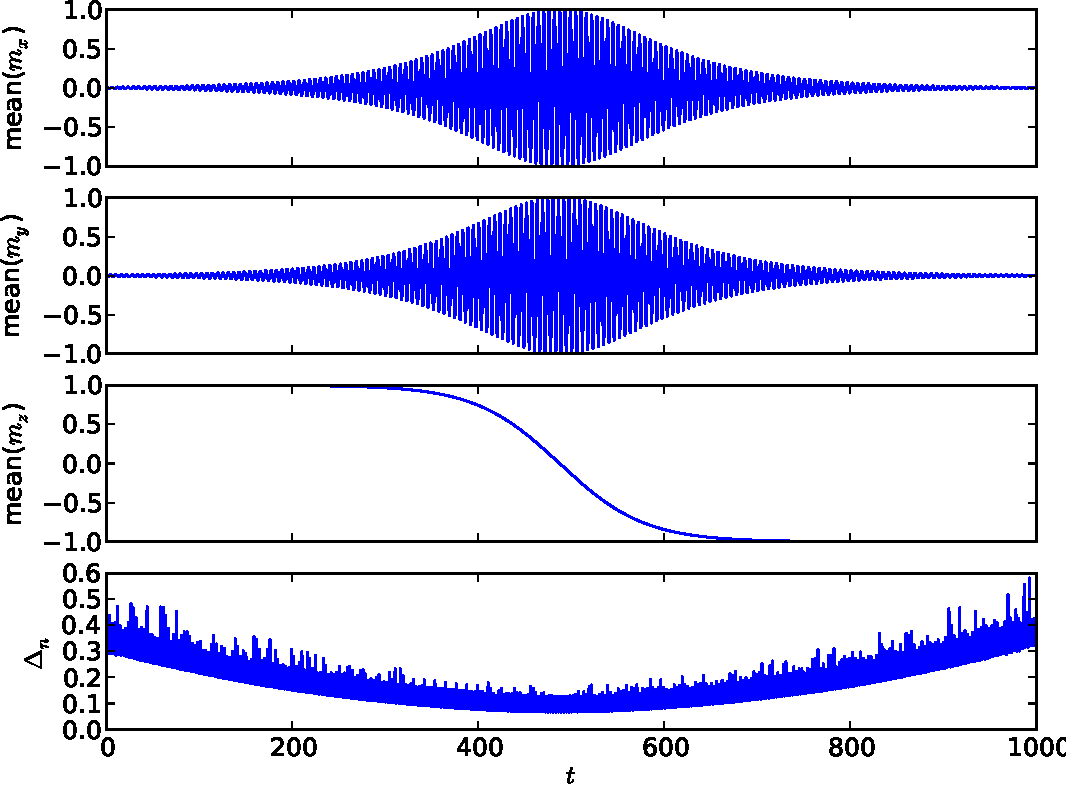
\includegraphics[width=0.8\textwidth]{plots/aimr-sphere-relax/imr0-meanmxsvs-meanmysvs-meanmzsvs-dtsvstimes.pdf}
  \caption{Plot of $\mv$ and $\dtn$ over time for the relaxing nano-sphere problem solved by adaptive IMR.}
  \label{fig:imr-llg-ode}
\end{figure}

The behaviour of the magnetisation and the time step selection using the adaptive IMR algorithm developed in \thisref{sec:adaptive-imr} is shown in \cref{fig:imr-llg-ode}.
The solutions given by adaptive BDF2 and TR (with $\abs{\mv}$ re-normalised after each time step)  are shown in \cref{fig:bdf2-llg-ode,fig:tr-llg-ode} respectively.
The overall behaviour of the IMR time step selection algorithm is seen to be working as expected: large steps are chosen at the start when very little switching occurs, the step size decreases as switching occurs and finally grows again as the switching finishes.

The small periodic peaks in the time step size are due to the precession: in Cartesian form (but not in the spherical polar coordinate form \cref{eq:79}) the precessional part of the solution is written as a sin/cosine term.
This causes periodic oscillations in the LTE.

Note, from \cref{fig:bdf2-llg-ode}, that the switching time obtained by BDF2 with the same error tolerances is very different to that given by IMR or TR, .
This is due to BDF2's spurious numerical damping (see \cref{sec:numerical-damping}), which initially moves the solution towards the unstable fixed point at $\mv=[1, 0, 0]$.
The accuracy of the TR solution is (qualitatively) good.
The time steps selected by the three algorithms are similar, TR selects slightly larger steps as would be expected due to its lower local truncation error (see \cref{sec:deriv-local-trunc}).


\begin{figure}
  \centering
  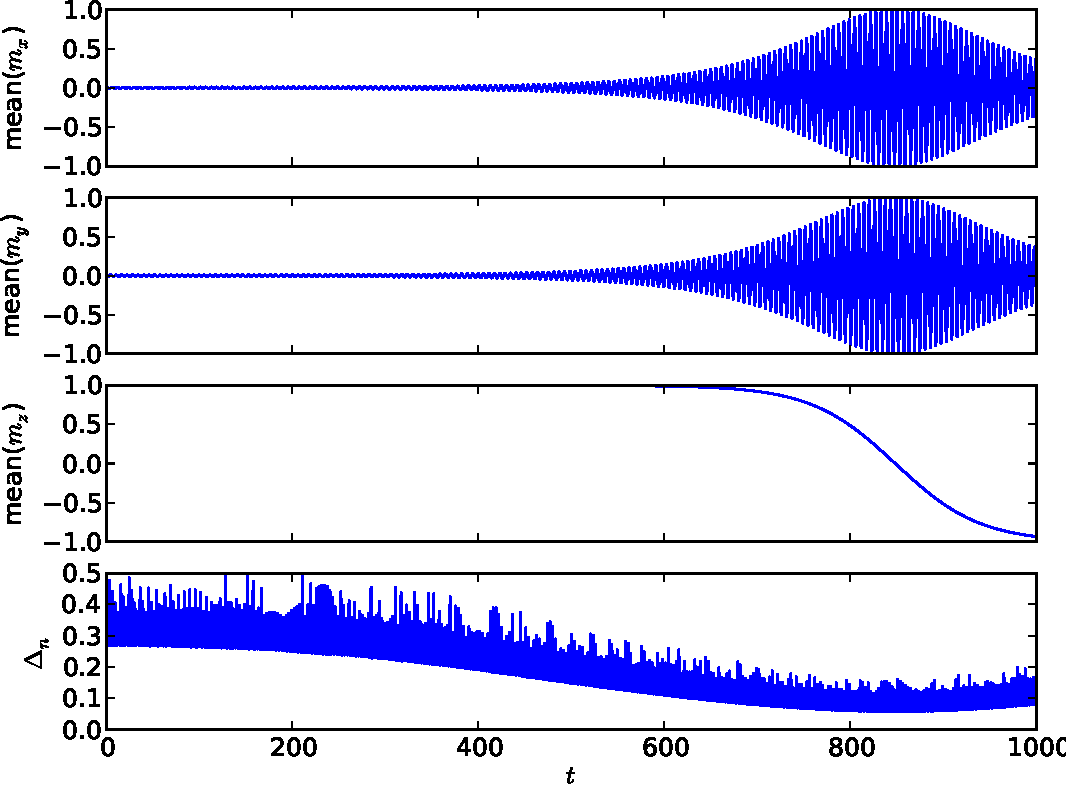
\includegraphics[width=0.8\textwidth]{plots/aimr-sphere-relax/bdf21-meanmxsvs-meanmysvs-meanmzsvs-dtsvstimes.pdf}
  \caption{Plot of $\mv$ and $\dtn$ over time for the relaxing nano-sphere problem solved by adaptive BDF2.}
  \label{fig:bdf2-llg-ode}
\end{figure}


\begin{figure}
  \centering
  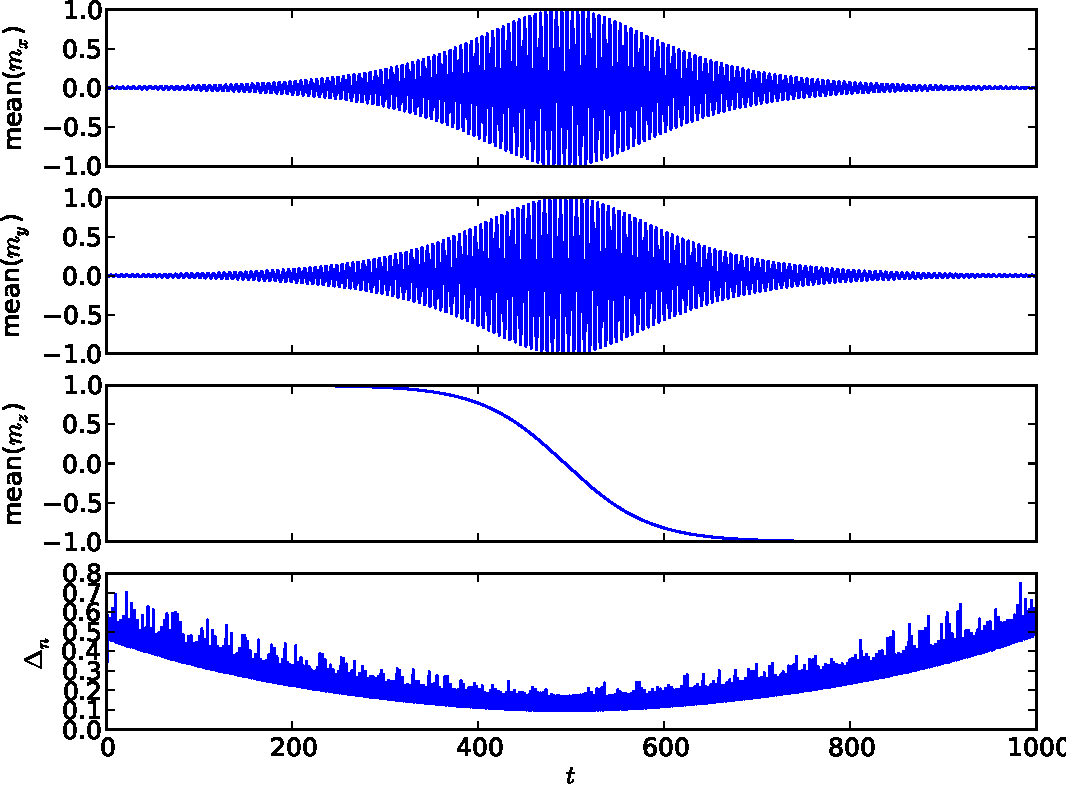
\includegraphics[width=0.8\textwidth]{plots/aimr-sphere-relax/tr1-meanmxsvs-meanmysvs-meanmzsvs-dtsvstimes.pdf}
  \caption{Plot of $\mv$ and $\dtn$ over time for the relaxing nano-sphere problem solved by adaptive TR.}
  \label{fig:tr-llg-ode}
\end{figure}

The behaviour of the magnetisation length over time is shown in \cref{fig:ml-aimr-ode}.
The maximum error when IMR is used is $\abs{\abs{\mv} -1} \approx 10^{-12}$, which is consistent with the Newton tolerance.
In contrast the error in the magnetisation length with the TR and BDF2 schemes reaches $\sim 10^{-2}$.

To investigate the effects of parameters on the magnetisation length conservation the experiment was run with varying $\dampc=1, 0.1, 0.01$, $\toltt = 5\times 10^{-3}, 10^{-3}, 5\times10^{-4}, 10^{-4}, 5\times10^{-5}, 10^{-5}$ and $\ntol=10^{-12}, 10^{-10}, 10^{-8}, 10^{-6}$.
A scatter plot showing the error in the length against the maximum (over time) converged Newton residual norm is shown in \cref{fig:ml-aimr-newton}.
We see that the magnetisation length conservation behaviour of IMR is well controlled by setting the Newton tolerance even with large variations in the time integration tolerance and damping parameter.

\begin{figure}
  \centering
  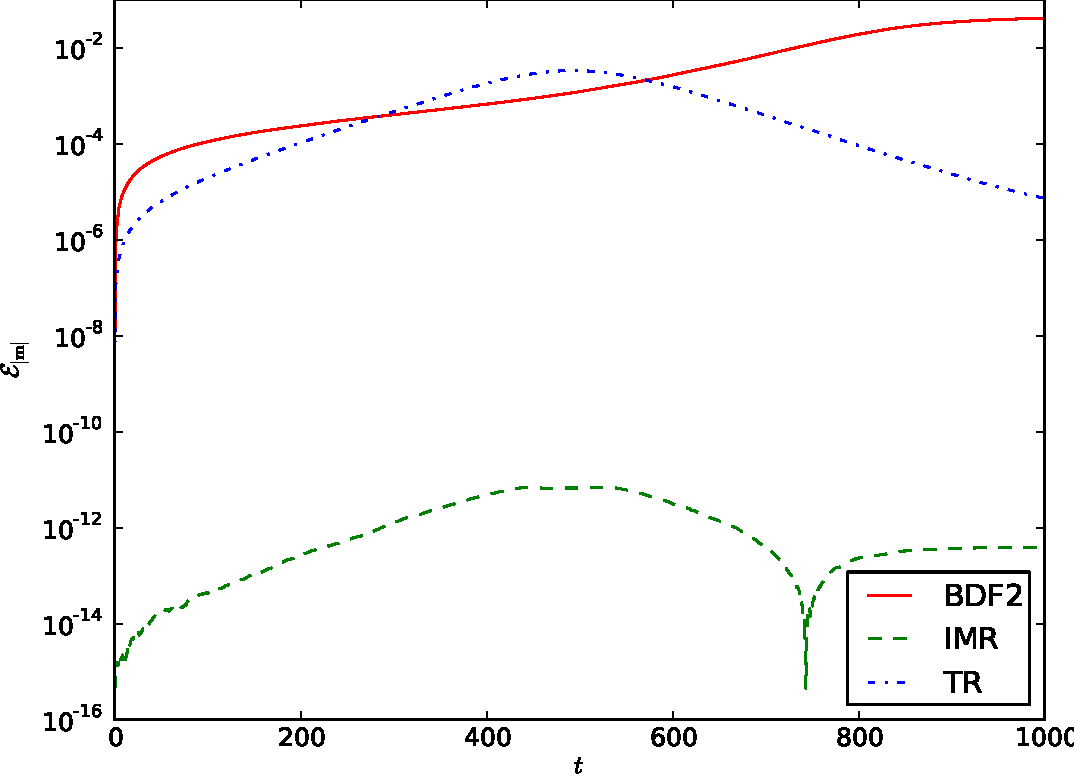
\includegraphics[width=0.8\textwidth]{plots/ode_llg_adaptive_ml/mlengtherrormaxesvstimes}
  \caption{Plot of magnetisation length errors, $\abs{\abs{\mv} -1}$, over time for the relaxing nano-sphere problem solved with each of the three adaptive integrators (without re-normalisation of $\mv$).}
  \label{fig:ml-aimr-ode}
\end{figure}

\begin{figure}
  \centering
  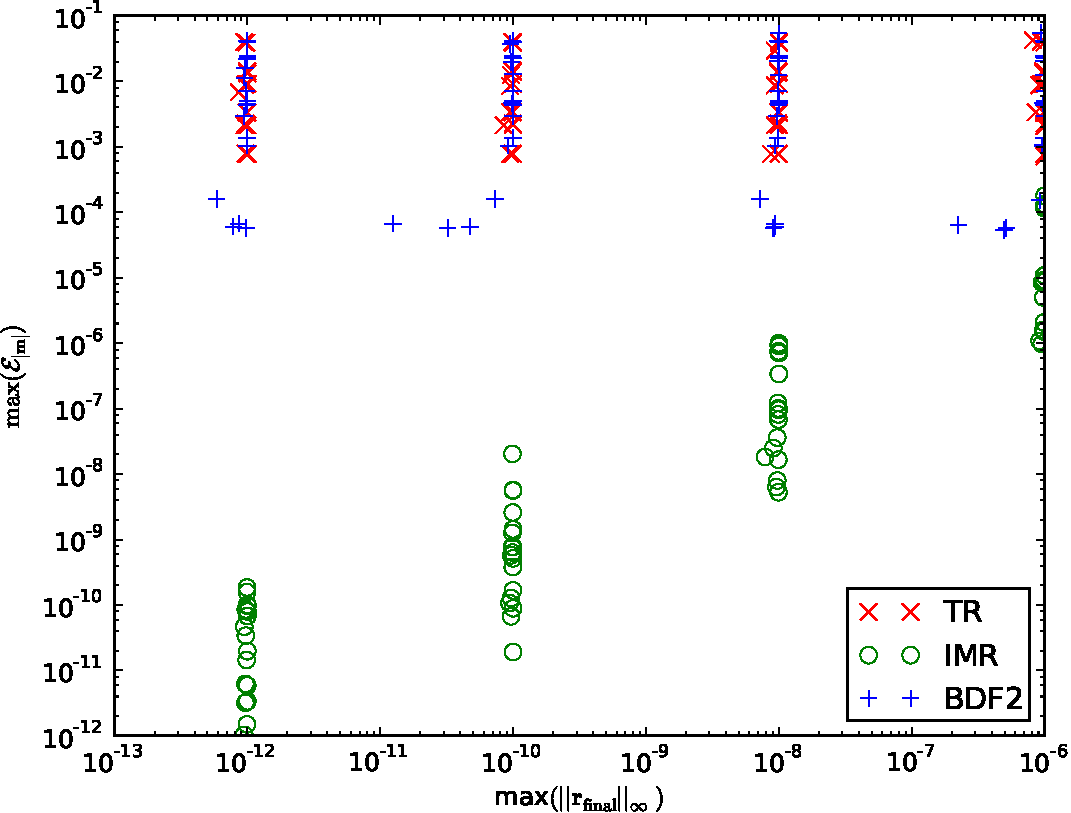
\includegraphics[width=0.8\textwidth]{plots/aimr_ode_llg_ml_sweep/maxofmlengtherrormaxesvsmaxminofnewtonresiduals.pdf}
  \caption{Plot of magnetisation length errors, $\abs{\abs{\mv} -1}$, against the maximum (over time) converged Newton residual norm a wide range of $\dampc$, $\ntol$ and $\toltt$ parameters.}
  \label{fig:ml-aimr-newton}
\end{figure}

The behaviour of the maximum error in the energy when $\dampc = 0$ as the adaptive step tolerance is reduced is shown in \cref{fig:energy-aimr-ode}.
The energy error for BDF2 without normalisation is very small (around the Newton tolerance), but when re-normalisation is used the error in energy increases drastically.
This is due to the injection/removal of energy when the magnetisation length is modified.
The energy error when using the TR/IMR algorithm (recall that, in this example TR and IMR are identical) is below the minimum value that can be calculated using floating point arithmetic.
This is not surprising as we expect it to be significantly smaller than the energy error of BDF2, which is $\sim 10^{-14}$ and it is calculated as the difference of two values of $\order{1}$ (so it cannot be calculated if it is smaller than $\sim 10^{-16}$).
% I also tried it with larger precession (ie m further from z) and nothing changes, leave it like this for simplicity.

\begin{figure}
  \centering
  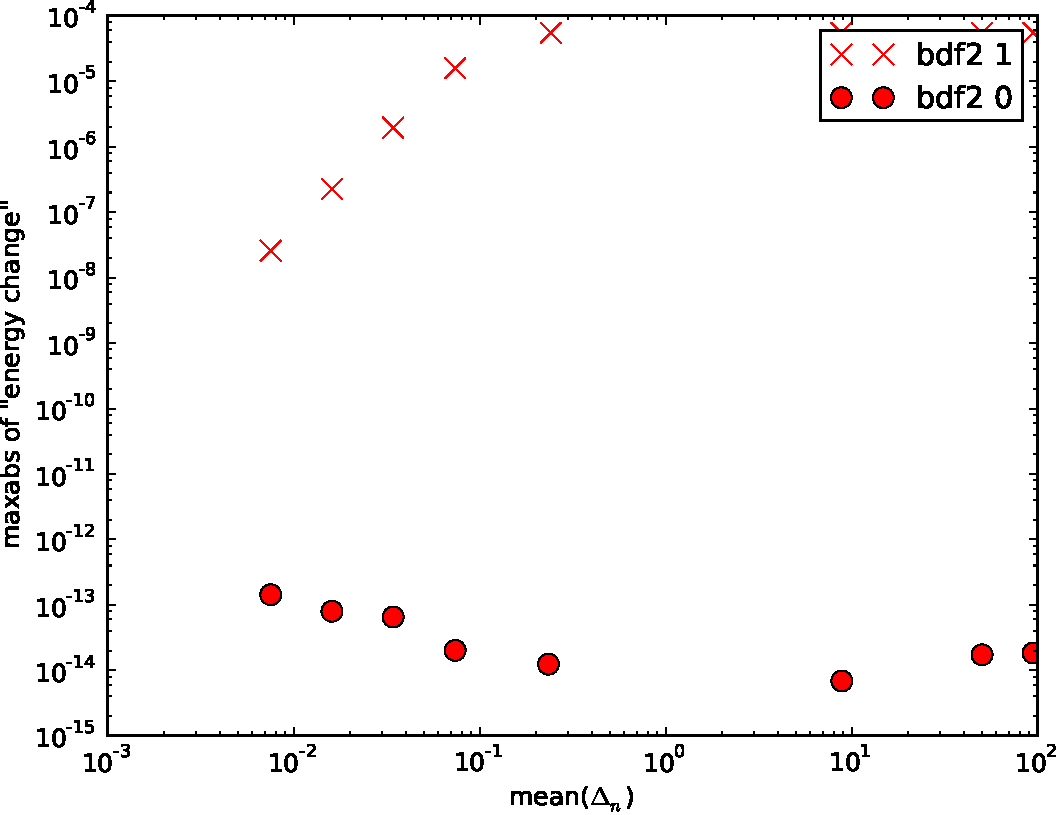
\includegraphics[width=0.8\textwidth]{plots/ode_llg_adaptive_energy/maxabsofenergychangevsmeanofdts}
  \caption{Convergence plot of the maximum error in the energy for the relaxing nano-sphere problem with $\dampc = 0$ solved using BDF2 with and without re-normalisation of $\mv$ (indicated in the legend by the digit 1 or 0 respectively). The energy error when using IMR is too small to be calculated.}
  \label{fig:energy-aimr-ode}
\end{figure}

\begin{figure}
  \centering
  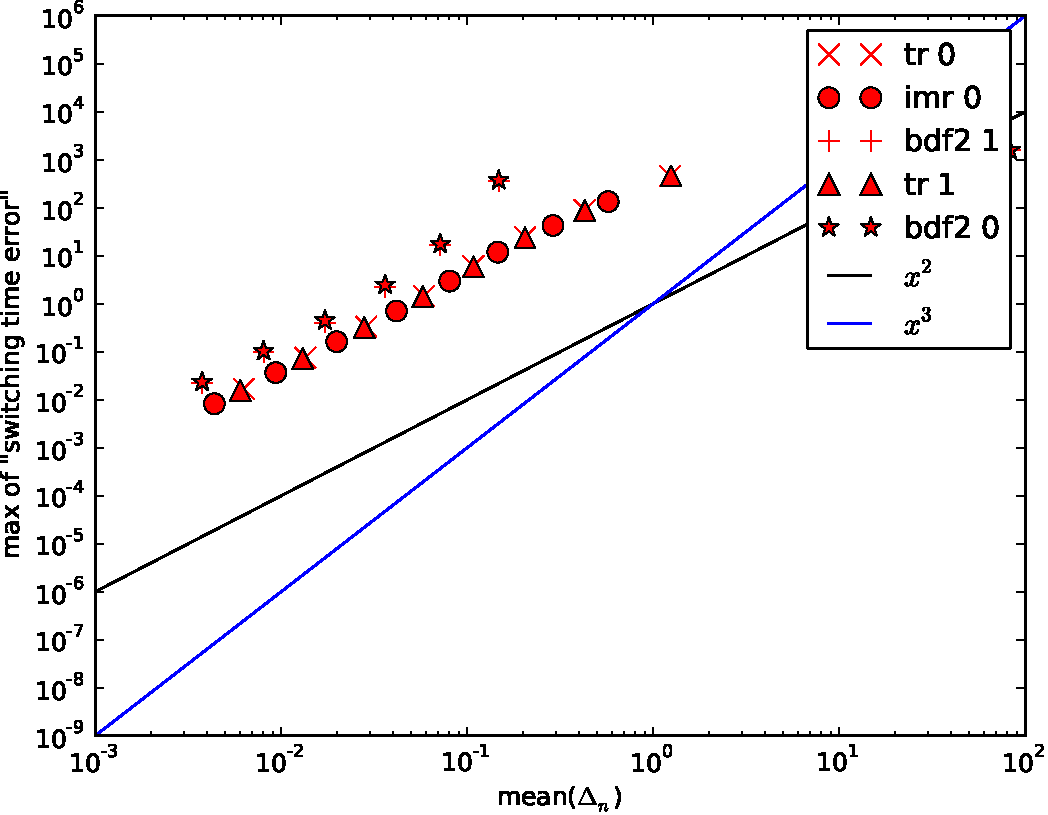
\includegraphics[width=0.8\textwidth]{plots/ode_llg_adaptive_convergence/maxofswitchingtimeerrorvsmeanofdts}
  \caption{Convergence plot of the switching time error, \cref{eq:sw-time-error}, against average time step for each method. The digit 1 or 0 indicates re-normalisation or no re-normalisation respectively.}
  \label{fig:llg-ode-convergence-swtime}
\end{figure}


Finally, we show convergence plots with respect to the two error norms.
\Cref{fig:llg-ode-convergence-swtime,fig:llg-ode-convergence-m} show the convergence with respect to the switching time error, $\swtimeerr$, and the global error, $\merr$, respectively.
Adaptive TR and BDF2 algorithms both with and without re-normalisation of the magnetisation after
each step are shown, along with the adaptive IMR algorithm developed in \thisref{sec:adaptive-imr}.


In \cref{fig:llg-ode-convergence-swtime} the convergence (in $\swtimeerr$) rates for TR and IMR are flat as would be expected from the asymptotic predictions, BDF2 does not attain this asymptotic convergence state until a comparatively small time step.
The maximum errors are around $1000$ time units, a relative error of $\sim 100\%$.
The errors of TR and IMR are extremely similar for a given mean time step size.
Once the asymptotic convergence regime is reached BDF2 has roughly three times the error of the other methods.
Note that the re-normalisation of $\mv$ in BDF2 and TR has only a minimal effect on their global error.
This indicates that length conservation property of IMR is unlikely to be providing a major benefit to the global error in this simple example.


In \cref{fig:llg-ode-convergence-m} all convergence (in $\merr$) rates show a kink around $\mean(\dtn) = 0.1$.
This is because $\abs{\mv} \approx 1$ and the error norm $\merr$ cannot be worse than the anti-parallel case.\footnote{A more effective error norm for such large error cases would be to use polar coordinates and track the total azimuthal angle passed through during the simulation. However: 1) this is non-trivial to implement in general; 2) some rescaling would be required to prevent the accumulated $\varphi$ error contribution from dominating that of $\theta$; and 3) we are not very interested in cases where the solution is highly inaccurate anyway.}
Above the kink the azimuthal angle is inaccurate and so the error norms are meaningless, below the kink the usual convergence behaviour can be seen.
Comparing the error norms different methods we see the same relationships as in \cref{fig:llg-ode-convergence-swtime}: BDF2 has three times the error and re-normalisation has little effect.


Note that TR consistently chooses larger time steps than IMR despite having similar global errors.
This may indicate that the LTE of IMR is indeed larger than that of TR (as is expected), but that the geometric integration properties of IMR reduce the build up of global error.
Alternatively it may be due to differing accuracies in the LTE estimate.


% Note that there are fewer visible points on \cref{fig:llg-ode-convergence-swtime,fig:llg-ode-convergence-m} for BDF2 than the other two methods, this is because at larger tolerances BDF2 takes overly large time steps (and has large global errors to match).
% Hence some points for BDF2 do not fit on the same scale (for these missing points: $\mean(\dtn) \approx 10\dash 100$, $\swtimeerr \approx 1000$ \ie a relative error of $100\%$, $\merr \approx 2$).
% This is consistent with the qualitatively wrong results given by BDF2 in \cref{fig:bdf2-llg-ode}.

\begin{figure}
  \centering
  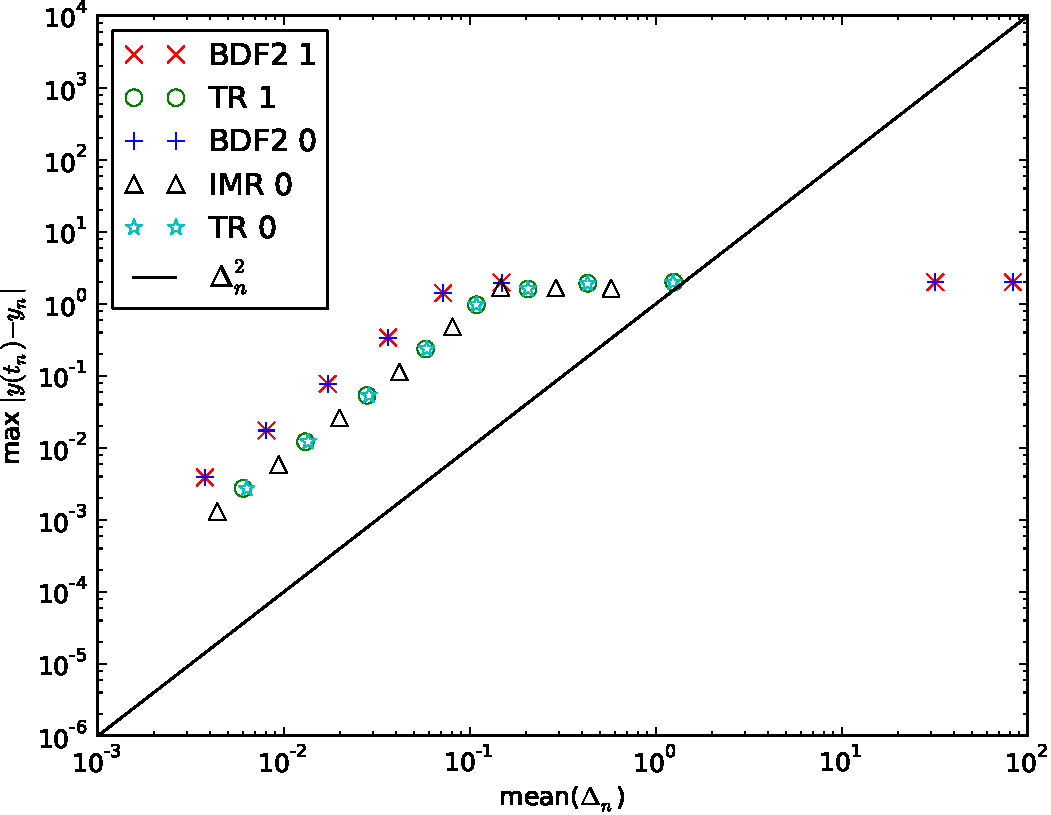
\includegraphics[width=0.8\textwidth]{plots/ode_llg_adaptive_convergence/maxoferrornormsvsmeanofdts}
  \caption{Convergence plots of the error in magnetisation, \cref{eq:m-sphere-error}, against average time step for each method. The digit 1 or 0 indicates re-normalisation or no re-normalisation respectively.}
  \label{fig:llg-ode-convergence-m}
\end{figure}

\section{Conclusions}

We have implemented an efficient algorithm for adaptive time step selection with the implicit midpoint rule.
The algorithm has been tested on a number of ODEs and found to choose similar time steps to other second order time integrators.
We have also demonstrated robustness in stiff problems and correct behaviour even when order reduction phenomena are encountered.

When applied to an ODE form of the LLG the adaptive IMR algorithm conserves $\abs{\mv}$ as expected for a wide variety of parameters, but the example used here is to be too simple for the energy property to be studied.
It also appears to give smaller global error norms than would be expected from its local truncation error, this may be due to the geometric integration properties.
Any effects of these geometric integration properties would be expected to be greatly amplified when solving ODE problems with many interacting spins or PDE problems.
This scenario will be tested in \cref{cha:numer-experiments} where the adaptive IMR algorithm is combined with the PDE methods discussed in other chapters.

Finally, we have observed some interesting results on the suitability of certain time integration methods to the simulation of the LLG equation.
We have found that the use of BDF2 results in significantly larger errors in the calculated switching time than the TR or IMR methods, particularly when the full precessional behaviour is not resolved.
We have also found that the process of re-normalising the magnetisation length after each time step in BDF2 methods greatly increases the error in the energy.


%%% Local Variables:
%%% mode: latex
%%% TeX-master: "./main"
%%% End:
